\documentclass[10pt, a4paper]{article}

\usepackage[utf8]{inputenc}
\usepackage[spanish]{babel} 
\usepackage[margin = 1in]{geometry} 
\usepackage{caratula}
\usepackage{algorithmicx}
\usepackage{algpseudocode}
\usepackage[Algoritmo]{algorithm}
\usepackage[fleqn]{amsmath}
\usepackage{amssymb}
\usepackage{color}
\usepackage{url}
\usepackage[colorlinks = true, linkcolor = blue]{hyperref}
\usepackage{comment}
\usepackage{hyperref}
\usepackage{ dsfont }
\usepackage{multirow}
\usepackage{listings}
\usepackage{listingsutf8}
\usepackage{color}

\usepackage{wrapfig}
\usepackage{nccmath}
\usepackage{caption}
\usepackage{subcaption}
\usepackage{amsthm}

\theoremstyle{definition}
\newtheorem{definition}{Definición}[section]
\newtheorem{theorem}{Teorema}

\definecolor{codegreen}{rgb}{0,0.6,0}
\definecolor{codegray}{rgb}{0.5,0.5,0.5}
\definecolor{codepurple}{rgb}{0.58,0,0.82}
\definecolor{backcolour}{rgb}{0.95,0.95,0.92}

\lstset{inputencoding=utf8/latin1,
  language=C++,
  basicstyle=\ttfamily,
  keywordstyle=\bfseries\color{blue},
  stringstyle=\color{red}\ttfamily,
  commentstyle=\color{mygreen}\ttfamily,
  morecomment=[l][\color{magenta}]{\#},
  % numbers=left,
  numberstyle=\color{gray},
  backgroundcolor=\color{backcolour},   
  keywordstyle=\color{magenta},
  breakatwhitespace=false,
  breaklines=true,
  captionpos=b,
  keepspaces=true,
  numbersep=5pt,
  showspaces=false,
  showstringspaces=false,
  showtabs=false,
  tabsize=3,
  inputencoding=utf8/latin1
}

% Para que tenga acentos el environment lstlisting
\lstset{
     literate=%
         {á}{{\'a}}1
         {í}{{\'i}}1
         {é}{{\'e}}1
         {ý}{{\'y}}1
         {ú}{{\'u}}1
         {ó}{{\'o}}1
         {ě}{{\v{e}}}1
         {š}{{\v{s}}}1
         {č}{{\v{c}}}1
         {ř}{{\v{r}}}1
         {ž}{{\v{z}}}1
         {ď}{{\v{d}}}1
         {ť}{{\v{t}}}1
         {ň}{{\v{n}}}1                
         {ů}{{\r{u}}}1
         {Á}{{\'A}}1
         {Í}{{\'I}}1
         {É}{{\'E}}1
         {Ý}{{\'Y}}1
         {Ú}{{\'U}}1
         {Ó}{{\'O}}1
         {Ě}{{\v{E}}}1
         {Š}{{\v{S}}}1
         {Č}{{\v{C}}}1
         {Ř}{{\v{R}}}1
         {Ž}{{\v{Z}}}1
         {Ď}{{\v{D}}}1
         {Ť}{{\v{T}}}1
         {Ň}{{\v{N}}}1                
         {Ů}{{\r{U}}}1    
}

\hypersetup{urlcolor=blue}

\makeatletter
\newenvironment{breakablealgorithm}
  {% \begin{breakablealgorithm}
   \begin{center}
     \refstepcounter{algorithm}% New algorithm
     \hrule height.8pt depth0pt \kern2pt% \@fs@pre for \@fs@ruled
     \renewcommand{\caption}[2][\relax]{% Make a new \caption
       {\raggedright\textbf{\ALG@name~\thealgorithm} ##2\par}%
       \ifx\relax##1\relax % #1 is \relax
         \addcontentsline{loa}{algorithm}{\protect\numberline{\thealgorithm}##2}%
       \else % #1 is not \relax
         \addcontentsline{loa}{algorithm}{\protect\numberline{\thealgorithm}##1}%
       \fi
       \kern2pt\hrule\kern2pt
     }
  }{% \end{breakablealgorithm}
     \kern2pt\hrule\relax% \@fs@post for \@fs@ruled
   \end{center}
  }
\makeatother

\newcommand{\bigo}[1]{\ensuremath{\mathcal{O}(#1)}}

\begin{document}

\titulo{Trabajo práctico}

\subtitulo{\textit{Extended Formulations and Branch-and-Cut Algorithms for the Black-and-White Traveling Salesman Problem}}

\materia{Seminario Avanzado de Programación Lineal Entera}

\integrante{Bogdanich Espina, Vera}{601/14}{verabogdanichespina@gmail.com}
\integrante{Puterman Colomer, Lucas}{830/13}{lucasputerman@gmail.com}

\maketitle

\tableofcontents

\newpage

\section{Introducción}

\subsection{Problema del Viajante de Comercio Blanco y Negro}
En este trabajo$^{\cite{main}}$ estudian una variante del problema del viajante de comercio: \textit{el problema del viajante de comercio blanco y negro}, o BWTSP por \textit{black-and-white travelling salesman problem}.

El BWTSP está definido sobre un grafo no dirigido $G = (V,E)$ que tiene su conjunto de vértices divido en dos, $V = B \cup W$, los blancos W y los negros B. Además, cada arista $e \in E$ tiene una distancia $d_e \in \mathds{N}$ y un costo $c_e \in \mathds{N}$ asociado. El objetivo es encontrar el camino de longitud mínima que recorre todos los vértices, y en el que el trayecto entre dos nodos negros consecutivos contiene a lo sumo Q nodos blancos y tiene una distancia de L como máximo. En la figura \ref{fig:ejemplo_bwtsp} se puede ver una instancia del problema junto con su solución.

\begin{figure}[H]
    \centering
    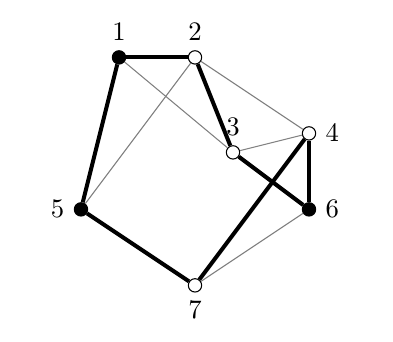
\includegraphics[width=0.4\textwidth]{ejemplo_bwtsp.png}
    \caption{Una instancia con B = \textbraceleft 1, 5, 6\textbraceright, W = \textbraceleft 2, 3, 4, 7\textbraceright, y una solución factible indicada por las aristas gruesas para Q = 2 y L = 3. La solución es óptima, por ejemplo, cuando el costo y la distancia de cada arista es 1 para todas las contenidas en la solución, y 2 para el resto.}
    \label{fig:ejemplo_bwtsp}
\end{figure}

Entre las aplicaciones de este problema están las operaciones aéreas de trayectos cortos. En este caso los vértices negros pueden representar estaciones de mantenimiento que los aviones tienen que visitar después de Q + 1 tramos como máximo, o después de haber recorrido una distancia máxima de L.

BWTSP es un problema NP-Hard por lo que es atacado mediante optimización combinatoria para encontrar soluciones exactas.

\subsection{Conceptos de Programación Lineal Entera}

Un programa entero (PE) es un problema de optimización que tiene la pinta:
$$min_{x \in X} c^Tx$$
Donde $X = \mathds{Z}^n\ \cap\ \{x \in \mathds{R}^n\ |\ Ax \leq b \}$ con alguna matriz $A$ y vector $b$. El poliedro $\{x \in \mathds{R}^n\ |\ Ax \leq b \}$ se llama una \textit{formulación} del conjunto $X$.
Un PE tiene varias formulaciones posibles, por ejemplo, en la figura \ref{fig:ejemplo_formulaciones}, las lineas sólidas y punteadas contienen al mismo conjunto de puntos enteros, es decir, los poliedros correspondientes son formulaciones del mismo conjunto.
Dados dos poliedros $P$ y $Q$, ($P \cap \mathds{Z}^n = Q \cap \mathds{Z}^n$) decimos que $P$ es una formulación \textit{más fuerte} o \textit{mejor} que $Q$ si $P \subsetneq Q$.

\begin{figure}[H]
  \centering
  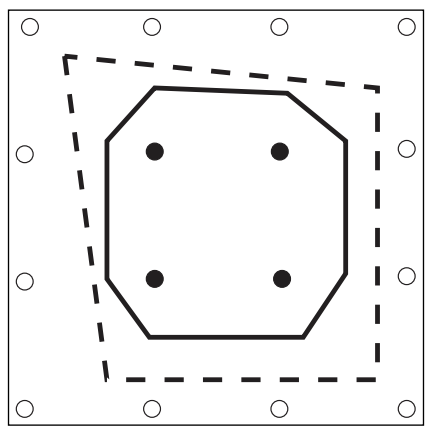
\includegraphics[width=0.4\textwidth]{ejemplo_formulaciones.png}
  \caption{Dos formulaciones del mismo conjunto.}
  \label{fig:ejemplo_formulaciones}
\end{figure}

Llamaremos \textit{región factible} al conjunto de las \textit{soluciones factibles}, es decir, el conjunto de todos los posibles puntos (conjuntos de variables) que satisfacen las restricciones del problema. A su vez, llamaremos \textit{función objetivo} a la función $f(x)$ de variables $(x_1,\dots,x_n)$ sobre una región factible $X$. Luego, lo que buscamos es:
$$min_{x \in X} f(x)$$

En la práctica, formulaciones mejores del mismo problema usualmente pueden ser resueltas en tiempos menores. Para eso se buscan modelos nuevos del problema donde se añaden distintas \textit{restricciones} al espacio de soluciones. Este trabajo se basa en comparar distintas formulaciones de BWTSP.

Veamos como se aplica esto al BWTSP. Como veremos en detalle en la sección \ref{sec:modelo_base}, las distintas formulaciones del trabajo parten de un modelo basado en las variables de decisión $x_e \in \{0,1\}, \forall e \in E$ que indican si una arista se incluye en el ciclo. Básicamente, la función que buscaremos minimizar es la siguiente:
$$\min \sum_{e \in E} c_{e} x_{e}$$
Esto representa el conjunto de aristas de costo mínimo. Por supuesto que esto no es suficiente, ya que además debemos añadir las restricciones propias del BWTSP para indicar nuestro espacio de soluciones factibles, y estas son:
\begin{itemize}
  \item Los vértices seleccionados deben formar un ciclo hamiltoniano.
  \item Entre dos vértices negros visitados debe haber a lo sumo $Q$ vértices blancos (restricción de salto).
  \item El ciclo tiene una distancia $L$ como máximo (restricción de distancia).
\end{itemize} 

\subsubsection{Relajaciones Lineales}
Como fue mencionado previamente, $BWTSP$ pertenece a NP-Hard, por lo que no es posible atacarlo directamente, es por esto que se utilizan en la práctica, distintos métodos que hacen uso de \textit{relajaciones lineales}.

La técnica de relajación linear en un problema de programación lineal entera consiste en ignorar temporalmente la restricción de tener variables enteras. Por ejemplo, en programa entero 0-1, las restricciones tienen la pinta:
$$x_i \in \{0,1\}$$
Mientras que la relajación lineal del problema usa las siguientes restricciones:
$$0 \leq x_i \leq 1$$
La técnica de relajación convierte un problema de optimización NP-Hard en un problema relacionado que puede ser resuelto en tiempo polinomial. La solución obtenida con la relajación puede ser usada para ganar información sobre el problema original. 


\subsubsection{Branch and Cut}
Branch and cut, o ramificación y corte, es un método de optimización combinatoria para resolver problemas de programación lineal entera, en particular, es el método utilizado en el trabajo estudiado.

La idea detrás de este método, es usar una combinación del método de \textit{planos de corte} con algoritmos de \textit{branch and bound}. Estos métodos, funcionan resolviendo una secuencia de \textit{relajaciones lineales} del problema en enteros.

\subsubsection{Planos de corte}
La idea detrás del método de planos de corte es ir agregando restricciones a un programa lineal hasta que la solución óptima factible tenga valores enteros. Por supuesto, teniendo cuidado con las restricciones que se añaden para que no cambie el problema.

Llamaremos a las restricciones que se añaden, \textit{cortes}. Un corte relativo a una solución fraccional actual, debe satisfacer las siguientes condiciones:
\begin{itemize}
  \item Toda solución entera factible debe ser factible con el corte.
  \item La solución fraccionaria actual no debe ser factible con el corte.
\end{itemize}

En la figura \ref{fig:ejemplo_cut} se puede ver un ejemplo gráfico de un corte. El círculo rojo representa la solución óptima fraccionaria encontrada. Los círculos negros son las soluciones enteras y la línea roja representa un corte que cumple con ambos requisitos, acotando nuestro espacio de soluciones factibles.
\begin{figure}[H]
  \centering
  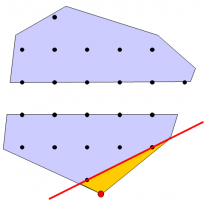
\includegraphics[width=0.4\textwidth]{ejemplo_cut.png}
  \caption{La linea roja representa un corte posible en una instancia.}
  \label{fig:ejemplo_cut}
\end{figure}

Hay dos formas de generar cortes. La primera, los cortes de Gomory, genera cortes para cualquier problema de programación lineal. Esta tiene la ventaja de “resolver"\ cualquier problema, pero la desventaja de que puede ser muy lento. El segundo enfoque, consiste en utilizar la estructura del problema que se quiere resolver para conseguir buenos cortes. De esta forma se pueden conseguir resultados muy buenos pero con la desventaja de tener que hacer un análisis para cada problema por separado.

\subsubsection{Branch and Bound}
El método Branch and Bound (B\&B) es una de las principales herramientas en la construcción de soluciones exactas para problemas de optimización.
Un algoritmo B\&B busca la solución en el espacio de soluciones completo de un problema.
Sin embargo, hacer una enumeración explicita de las soluciones es imposible debido a que el número de posibles soluciones es exponencialmente creciente.
El uso de cotas combinadas con el valor de la mejor solución actual, permite al algoritmo buscar partes de la solución implícitamente.
En cualquier punto durante el algoritmo, el estado de la solución con respecto a la búsqueda del espacio de soluciones es descripto por una serie de subconjuntos inexplorados del espacio de soluciones junto con la mejor solución encontrada hasta el momento.
Inicialmente, solo un subconjunto existe (el espacio de solución completo) y la mejor solución hallada es $\infty$. 
Los subespacios no explorados se representan como nodos en un árbol de búsqueda generado dinámicamente, que inicialmente solo contiene la raíz. 
En cada paso de una iteración de B\&B se procesa un nodo.

Un algoritmo de B\&B se puede dividir en dos partes:

\begin{itemize}
  \item Ramificación (branching): Dividir recursivamente el espacio de búsqueda actual y minimizar la función objetivo en los espacios resultantes.
  \item Acotación (bounding): Como la ramificación en si misma implicaría una enumeración completa del espacio de búsqueda, se descartan ramas basadas en cotas de soluciones actuales del algoritmo.
\end{itemize}

Cada iteración consta de tres componentes principales:
 
\begin{itemize}
  \item Selección del nodo a procesar.
  \item Calculo de cotas (bound).
  \item Ramificación (branching).
\end{itemize}

En la figura \ref{fig:ejemplo_bandb} la situación inicial y el primer paso de un proceso de B\&B es ilustrado. Notar que los nodos $S1$ y $S4$ se cierran ya que dada la solución actual de ese momento ya se sabe que el resultado óptimo no se entcontrará en esos espacios.

El orden en que los componentes de la iteración son ejecutados puede variar según la estrategia utilizada para seleccionar el siguiente nodo a procesar.
Si la selección del siguiente subproblema está basada en el valor de la cota de los subproblemas, entonces la primera operación en una iteración luego de elegir un nodo es ramificar.
Por ejemplo, en una subdivisión del espacio de solución de un nodo en dos o mas subespacios a ser investigados en iteraciones posteriores.
Para cada uno de estos, se revisa si el subespacio consiste de una sola solución en cuyo caso se compara con la mejor solución actual y se guarda la mejor.
Si se puede establecer que el subespacio no contiene la solución óptima, se descarta. En caso contrario, se guarda con los nodos a revisar junto con su cota.
 
\begin{figure}[H]
  \centering
  \includegraphics[width=0.7\textwidth]{ejemplo_bandb.png}
  \caption{Ilustración del espacio de búsqueda de Branch and Bound.}
  \label{fig:ejemplo_bandb}
\end{figure}

\section{Modelo base}
\label{sec:modelo_base}

En la sección anterior, se vio una introducción a las herramientas utilizadas en este trabajo y se formularon coloquialmente las restricciones necesarias para modelar BWTSP. Veamos ahora una formulación genérica que servirá de base para los distintos modelos a introducirse en las secciones a venir.

Las variables de decisión $x_e \in \{0,1\}, \forall e \in E$ indican si una arista es incluida en el ciclo.
\begin{align} 
	\min & \sum_{e \in E} c_{e} x_{e} & \label{eq:1} \\
	\text {tal que} & \quad x(\delta(i))=2 & \forall i \in V \label{eq:2} \\
	& x(E(S)) \geq 2 & \forall S \subseteq V \backslash\{1\},\ S \neq \emptyset \label{eq:3} \\
	& \left\{e \in E : x_{e}=1\right\} & \text { satisface la restricción de salto para el camino después de cada } k \in B \label{eq:4} \\
	& \left\{e \in E : x_{e}=1\right\} & \text { satisface la restricción de distancia para el camino después de cada } k \in B \label{eq:5} \\
	& \mathbf{x} \in\{0,1\}^{|E|} & \label{eq:6}
\end{align}

Existen distintas formas de modelar ciclos hamiltonianos. En el trabajo estudiado se usan restricciones en el grado de los vértices \ref{eq:2} y el conjunto exponencial de restricciones de corte \ref{eq:3}. Se introduce la notación necesaria al final de esta sección.

Las restricciones \ref{eq:4} y \ref{eq:5} son modeladas de maneras distintas en las distintas formulaciones que serán vistas.

Por último, introducimos notación que se usó en las ecuaciones de este modelo, y/o que se va incluir en las próximas:

\begin{itemize}
	\item $A = \{(i,j)\ |\ \{i,j\} \in E\}$ obtenido al bidirijir el conjunto de aristas $E$.
	\item Para un subconjunto de vértices $S \subset V$, usaremos la notación $\delta(s) = \{\{i,j\} \in E\ |\ i \in S,\ j \notin S\}$,
$\delta^+(s) = \{\{i,j\} \in A\ |\ i \in S,\ j \notin S\}$ y $\delta^-(s) = \{\{i,j\} \in A\ |\ i \notin S,\ j \in S\}$.
	\item Para un conjunto de variables $\textbf{z}$ definidas en un conjunto $W$ y un subconjunto $W' \subseteq W$, se usará la notación $z(W') = \sum_{u \in W'} z_u$.
\end{itemize}

\section{Modelo de segmento del camino}

Hasta ahora solamente habíamos comentado un modelo base teórico, con restricciones abstractas que en la práctica deberían reemplazarse. En esta sección introducimos una formulación que se basa en la descripción del problema para determinar las restricciones abstractas. La idea de este modelo es identificar el camino desde un nodo $k \in B$ hasta el nodo negro siguiente sin indicar explícitamente cuál es. A este trayecto nos vamos a referir como “el camino asociado con el nodo $k$". Las variables $x_{i j}^{k} \in\{0,1\},\ \forall k \in B,\ \forall(i, j) \in A$ indican que la arista $(i,j)$ está contenida en el segmento del camino general asociada al vértice negro $k$. Con estas variables podemos modelar el segmento del camino asociada a cada nodo negro en las restricciones \ref{eq:7}–\ref{eq:10}, al igual que modelar las restricciones de salto y distancia, \ref{eq:4} y \ref{eq:5} respectivamente. A lo largo de este trabajo vamos a explicar en detalle las ecuaciones después de introducirlas.

\begin{align} 
	& x^{k}\left(\delta^{+}(k)\right)=1 & \forall k \in B \label{eq:7} \\
	& \sum_{j \in B \backslash\{k\}} x^{j}\left(\delta^{-}(k)\right)=1 & \forall k \in B \label{eq:8} \\
	& x^{k}\left(\delta^{-}(i)\right)=x^{k}\left(\delta^{+}(i)\right) & \forall k \in B,\ \forall i \in W \label{eq:9} \\
	& \sum_{k \in B} x_{i j}^{k}+x_{j i}^{k}=x_{e} & \forall e=\{i, j\} \in E \label{eq:10}
\end{align}

La ecuación \ref{eq:7} asegura que desde cada nodo negro sale una sola arista y que es parte de su segmento del camino. Mientras que la ecuación \ref{eq:8} garantiza que hacia cada nodo de $B$ llega una sola arista, y es parte del segmento del camino de un único nodo negro. Las restricciones de \ref{eq:9} indican que si la arista que llega a un nodo blanco pertenece al camino del nodo negro $k$ entonces la arista que sale de él también, y si no pertenece la que llega entonces la que parte tampoco. Por último, las restricciones \ref{eq:10} unen los dos conjuntos de variables: $x_{e}$ y $x_{i j}^{k}$, expresando que $(i,j)$ o $(j,i)$ son parte del segmento de algún $k$ sí y sólo sí la arista $e$ pertenece al camino final. Para que la formulación sea válida también hay que incluir las restricciones de salto y distancia, \ref{eq:11} y \ref{eq:12} en este caso.

\begin{align} 
	& \sum_{e=\{i, j\} \in E}\left(x_{i j}^{k}+x_{j i}^{k}\right) \leq Q+1 & \forall k \in B \label{eq:11} \\
	& \sum_{e=\{i, j\} \in E} d_{e}\left(x_{i j}^{k}+x_{j i}^{k}\right) \leq L & \forall k \in B \label{eq:12}
\end{align}

Llamamos PS, por \textit{path segment}, a la formulación resultante de reemplazar las restricciones abstractas \ref{eq:4} y \ref{eq:5} por \ref{eq:7}–\ref{eq:12} y las correspondientes a la definición de $x_{i j}^{k}$.

En el trabajo original también se incluye la restricción \ref{eq:13} que relaciona los trayectos asociados a cada nodo negro, asumiendo que $|B| \geq 3$:

\begin{align}
	& x^{k}\left(\delta^{-}(j)\right)+x^{j}\left(\delta^{-}(k)\right) \leq 1 & \forall k \neq j \in B \label{eq:13}
\end{align}

Esta restricción elimina ciclos al asegurar que si un nodo negro $j$ es el nodo negro inmediatamente siguiente a $k$ de $B$, entonces $k$ no puede estar inmediatamente después de $j$. Los resultados computacionales, que se introducen dentro de algunas secciones, muestran que estas desigualdades mejoran las cotas de PS para algunas instancias evaluadas, y a la variante del modelo que incluye \ref{eq:13} se la llama PS+.

\section{Formulaciones dependientes de la posición}

En el trabajo original, se analizan también, formulaciones dependientes del tiempo que proveen cotas fuertes. En general, y también en las formulaciones introducidas en esta sección, se agrega información sobre la posición (tiempo) de una arista en el circuito o en el segmento del camino asociado a un vértice negro.
De esta manera, aseguramos que la restricción de salto sea implícitamente satisfecha, pero con el costo de un significativamente mayor número de variables. En particular, si el límite de saltos no es muy grande, los algoritmos basados en estas formulaciones pueden producir resultados comparables con el estado del arte, o aún mejores.

Se introducirán tres formulaciones dependientes de la posición. La primera se basa en añadir información de la posición de una arista con respecto a su posición después del vértice negro anterior. Sin embargo, no se provee información explícita de cual es el vértice negro que inicializa cada segmento. Esto significa que las restricciones de distancia tienen que ser incluidas de una forma similar a la hecha anteriormente.

La segunda, puede ser vista como una reformulación dependiente de la posición de la formulación PS. Se agrega información sobre el vértice negro previo y la posición relativa es agregada en cada arista. Esta información nos permite modelar las restricciones de distancia.

Por último, una tercera forma de encarar el problema es una variante que puede ser vista como un modelo dependiente de la posición bidimensional. En lugar de especificar explícitamente el vértice negro que inicializa cada segmento, se provee información sobre la posición del segmento en el ciclo general junto con especificar la posición relativa de la arista en el segmento.
Sin perdida de la generalidad, se asume que un nodo arbitrario es elegido como el punto de partida de un ciclo y su segmento asociado se considera como el primer segmento.

Además, estas formulaciones dependientes de la posición se pueden interpretar con grafos en capas apropiadamente definidos. Estas interpretaciones ayudan a entender más profundamente la estructura de las soluciones en el espacio de variables extendidas y a encontrar mejores desigualdades válidas en el espacio extendido. Por lo tanto, se usará también este concepto al introducir las tres formulaciones.
La idea consiste en replicar los vértices originales una cantidad de veces en distintas capas y permiten asegurar de forma implícita las restricciones de saltos entre vértices negros consecutivos. Sin embargo, los detalles entre los grafos en capas utilizados en las distintas formulaciones difieren significativamente.

\subsection{Formulación dependiente de la posición pura}

Para esta formulación usamos las variables dependientes de la posición: $X^p_{ij} \in \{0,1\},\ \forall (i,j) \in A,\ \forall p \in \{1,2,\dots,Q+1\}$.
Para cada arista $(i,j) \in A$ la variable $X^p_{ij}$ es uno si y solo si esa arista está en las posición $p$ en el camino que empieza en el vértice negro previo. Como $p$ indica la posición en el segmento de camino previo y no en el ciclo general, más de una arista pueden estar en la misma posición $p$

\begin{align}
	& X^{1}\left(\delta^{+}(k)\right)=1 & \forall k \in B \label{eq:14} \\
	& \sum_{p=1}^{Q+1} X^{p}\left(\delta^{-}(k)\right)=1 & \forall k \in B \label{eq:15} \\
	& X^{p}\left(\delta^{-}(i)\right)=X^{p+1}\left(\delta^{+}(i)\right) & \forall i \in W,\ \forall p \in\{1,2, \ldots, Q\} \label{eq:16} \\
	& \sum_{p=1}^{Q+1}\left(X_{i j}^{p}+X_{j i}^{p}\right)=x_{e} & \forall e=\{i, j\} \in E \label{eq:17}
\end{align}

Primero veamos que podemos remover las restricciones de salto \ref{eq:4} ya que estas están implícitamente garantizadas por el rango de valores que puede tomar $p$.
Las restricciones (\ref{eq:14}-\ref{eq:16} nos hablan del balance del flujo de aristas en el espacio de las variables con indices por posición.
\begin{itemize}
  \item \ref{eq:14} indica que una arista sale de cada vértice negro en la posición uno.
  \item \ref{eq:15} dice que llega a cada vértice negro exactamente una arista que pertenece a un segmento de longitud a lo sumo $Q+1$.
  \item \ref{eq:16} establece que una arista puede salir de un vértice blanco $i$ en la posición $p+1$ si y solo si otra arista llega a ese mismo vértice en la posición $p$, es decir que los vértices blancos no son los últimos de un segmento.
\end{itemize}
Por último, \ref{eq:17} establece un vínculo entre las variables de aristas indexadas por la posición y las variables de aristas no dirigidas definidas previamente.

De esta forma tenemos bien definido nuestro concepto de segmento de camino, aunque sin especificar que vértice negro inicia cada segmento. Por lo tanto, se deben añadir restricciones de eliminación de caminos para eliminar todos los trayectos que violan la restricción de distancia.
Por lo tanto, $\mathcal{P}_{inf} \subset 2^E$ denota el conjunto de todos los caminos entre dos vértices negros en $G$ que no contienen vértices negros más adelante y que violan la restricción de distancia.
Es decir, $\sum_{e \in P} d_e > L, \forall P \in \mathcal{P}_{inf}$


\begin{align}
	& \sum_{e \in P} x_{e} \leq|P|-1 & \forall P \in \mathcal{P}_{\mathrm{inf}} \label{eq:18}
\end{align}

Llamamos PD a la formulación dependiente de la posición que se obtiene formalmente de la formulación genérica incluyendo las restricciones \ref{eq:14}-\ref{eq:18} y restricciones por definición para las variables dependientes de la posición $X_{ij}^p$ en lugar de las restricciones genéricas de distancia y salto \ref{eq:4} y \ref{eq:5} respectivamente.

Un conjunto polinomial de desigualdades que usualmente mejoran las cotas de las formulaciones dependientes del tiempo son las llamadas desigualdades de dos ciclos. Para el caso de PD, definimos las siguientes desigualdades:

\begin{align}
	& X_{i j}^{p} \leq \sum_{h \neq i} X_{j h}^{p+1} & \forall p \in\{1,2, \ldots, Q\},\ \forall e=\{i, j\} \in E, j \in W \label{eq:19} \\
	& X_{i j}^{p} \leq \sum_{h \neq i} X_{j h}^{1} & \forall p \in\{1,2, \ldots, Q+1\},\ \forall e=\{i, j\} \in E, j \in B \label{eq:20}
\end{align}

Estas simplemente dicen que si una arista $(i,j)$ está en la posición $p+1$ en un segmento dado, entonces la arista previa en la posición $p$ convergente al vértice $i$, no puede diverger del vértice $j$.
Llamamos a la variante de PD con las restricciones \ref{eq:19} y \ref{eq:20},  PD$^+$.

Como se introdujo previamente en esta sección, las formulaciones dependientes de la posición pueden ser vistas como formulaciones en un grafo en capas. Ahora, definimos el digrafo en capas $G_Q = (V_Q,A_Q)$ asociado a la formulación PD.
El conjunto de vértices $V_Q = \{i_0 | i \in B\} \cup \{i_p | i \in W,\ 1 \leq p \leq Q\}$ consiste de vértices negros en la capa cero (ya que la cuenta de saltos de cada segmento del camino se inicializa por un vértice negro con 0) y copias de los vértices blancos en todas las capas factibles $p, 1 \leq p \leq Q$. Un vértice $i_p$ incluido en una solución, indica que el único camino de $i$ al vértice negro que inicia su segmento, tiene longitud $p$.
Por lo tanto, en el espacio de $G_Q$, cualquier solución factible debe visitar todos los vértices negros (en la capa cero) y exactamente una copia de cada vértice blanco (en alguna capa $p, 1 \leq p \leq Q$).
El conjunto de aristas $A_Q$ consiste de:
\begin{itemize}
  \item aristas $(i_p,j_{p+1})$ entre dos vértices blancos $i$ y $j$,
  \item aristas $(i_0,j_0)$ entre dos vértices negros $i$ y $j$,
  \item aristas $(i_0,j_1)$ entre un vértice negro $i$ y un vértice blanco $j$, y
  \item aristas $(i_p,j_0)$ con $1 \leq p \leq Q$ entre un vértice blanco $i$ y un vértice negro $j$.
\end{itemize}

Formalmente: $A_Q = \{(i_p,j_{p+1})\ |\ i_p,j_{p+1} \in V_Q,\ (i,j) \in A\} \cup \{(i_0,j_0)\ |\ i,j \in B, (i,j) \in A\} \cup \{(i_p,j_0)\ |\ i \in W,\ j \in B,\ i_p \in V_Q (i,j) \in A\}$.

La interpretación de PD en el grafo $G_Q$ está basada en asociar cada una de las variables definidas previamente $X_{ij}^p$ ya se con la arista $(i_{p-1},j_p)$ si $j \in W$, o bien la arista $(i_{p-1},j_0)$ si $j \in B$.
La figura en \ref{fig:ejemplo_capas_q} muestra la solución de la figura \ref{fig:ejemplo_bwtsp} en el contexto del digrafo $G_Q$.

\begin{figure}[H]
  \centering
  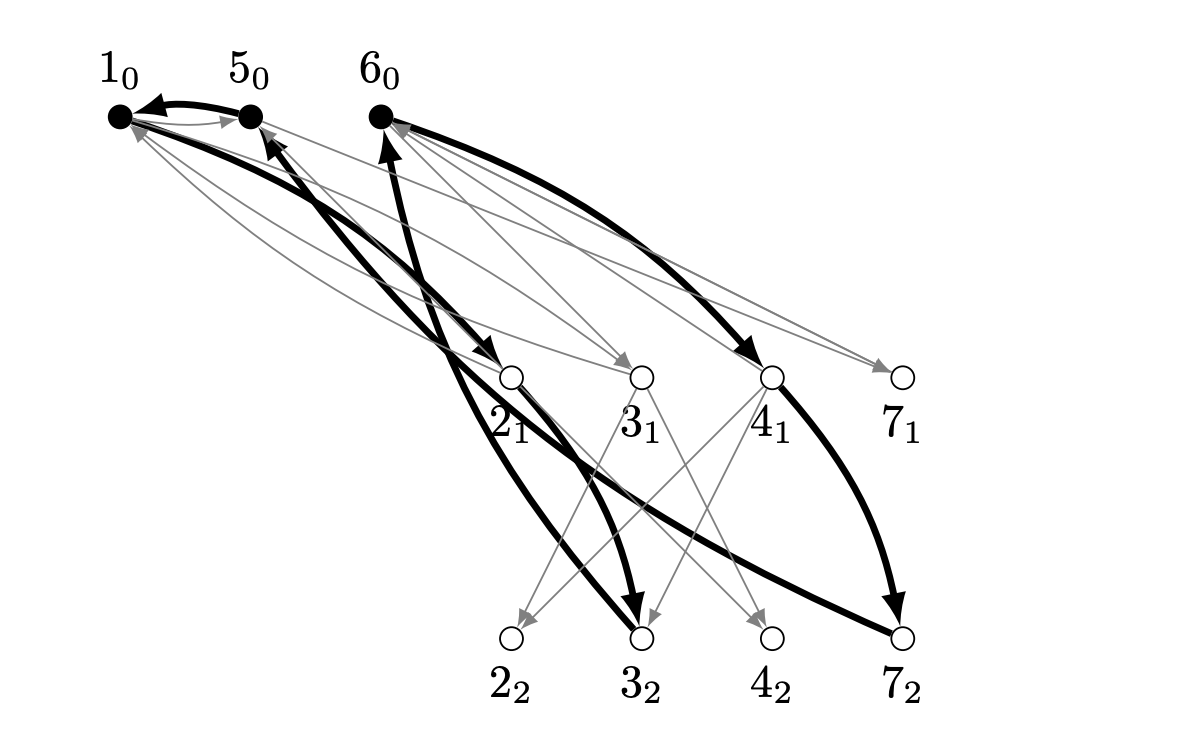
\includegraphics[width=0.7\textwidth]{ejemplo_capas_q.png}
  \caption{Digrafo en capas $G_Q = (V_Q,A_Q)$ correspondiente a la instancia dada en la figura \ref{fig:ejemplo_bwtsp}. Las aristas en negrita representan a la solución dada en esa figura.}
  \label{fig:ejemplo_capas_q}
\end{figure}

Hay varias desigualdades validas que mejoran significativamente las cotas de LP del modelo dependiente del tiempo y que son más fáciles de describir en términos del digrafo $G_Q$.
Se pueden considerar desigualdades de corte especificas para grafos en capas más generales que no corresponden con los $\textbf{x}$-cortes reescritos col las variables $X_{ij}^p$ vía las ecuaciones \ref{eq:17}.
Diferentes clases de estas desigualdades de corte pueden ser obtenidas de la observación de que todos los vértices deben ser alcanzables desde el vértice de salida $1_0$ que se asume, sin pérdida de la generalidad, como el comienzo del ciclo. 
El trabajo estudiado considera al conjunto de desigualdades \ref{eq:21} que asegura que al menos una arista debe cruzar cada corte, separando al conjunto de vértices negros de todas las copias de un vértice blanco dado.

\begin{align}
	& X\left(\delta^{-}(S)\right) \geq 1 & \forall S \subseteq V_{\mathrm{Q}} \backslash\left\{j_{0} : j \in B\right\}, \exists i \in W |\left\{i_{p}, p \in\{1,2, \ldots, Q\}\right\} \subseteq S \label{eq:21}
\end{align}

La variante de PD$^+$ que agrega estas últimas restricciones va a ser llamada PD$^{++}$.

\subsection{Reformulación del modelo de segmento del camino}

Se pueden incorporar las ideas del modelo dependiente de la posición anterior al modelo de segmento del camino. Las variables $Y_{i j}^{k, p} \in\{0,1\},\ \forall k \in B,\ \forall p \in\{1, \ldots, Q+1\},\ \forall(i, j) \in A$ van a indicar que el arco $(i,j)$ está en la posición $p$ del recorrido que empieza en el nodo $k$.

El modelo nuevo está compuesto por las restricciones iniciales, \ref{eq:22}-\ref{eq:25} para reemplazar a \ref{eq:7}-\ref{eq:10} que modelan los segmentos de camino, \ref{eq:14}-\ref{eq:17} del modelo anterior, y restricciones de distancia y salto que reemplazarían a las abstractas. Nos vamos a referir a esta formulación como PDPS.

\begin{align}
	& Y^{k, 1}\left(\delta^{+}(k)\right)=1 & \forall k \in B \label{eq:22} \\
	& \sum_{j \in B \backslash\{k\}} \sum_{p=1}^{Q+1} Y^{j, p}\left(\delta^{-}(k)\right)=1 & \forall k \in B \label{eq:23} \\
	& Y^{k, p}\left(\delta^{-}(i)\right)=Y^{k, p+1}\left(\delta^{+}(i)\right) & \forall k \in B, \forall i \in W, \forall p \in\{1, \ldots, Q\} \label{eq:24} \\
	& \sum_{k \in B} \sum_{p=1}^{Q+1}\left(Y_{i j}^{k, p}+Y_{j i}^{k, p}\right)=x_{e} & \forall e=\{i, j\} \in E \label{eq:25}
\end{align}

La ecuación \ref{eq:22} garantiza que una sola arista parte de cada nodo negro en la primera posición de su camino. Mientras que \ref{eq:23} asegura que una única arista llega a cada nodo negro, y que esa arista está asociada al segmento de un nodo negro distinto. Además, si en la posición $p$ se alcanza el nodo blanco $i$ entonces en la posición $p+1$ se tiene que salir de ese nodo, y los dos tramos tienen que pertenecer al camino del mismo nodo negro, como se indica en la ecuación \ref{eq:24}. Por último, como en los modelos anteriores, las restricciones \ref{eq:25} relacionan las variables nuevas con las del modelo base.

Al igual que en el modelo dependiente de la posición anterior, las restricciones de salto están satisfechas por el rango de $p$ con el que se definen las variables $Y$, mientras que las restricciones de distancia se pueden escribir así:

\begin{align}
	& \sum_{p=1}^{Q+1} \sum_{e=\{i, j\} \in E} d_{e}\left(Y_{i j}^{k, p}+Y_{j i}^{k, p}\right) \leq L & \forall k \in B \label{eq:26}
\end{align}

Como en todos los modelos que introdujimos hasta el momento, vamos a reforzar PDPS evitando ciclos para los dos tipos de vértices, como se indica en las ecuaciones \ref{eq:27} y \ref{eq:28}, generando PDPS$^{+}$.

\begin{align}
	& Y_{i j}^{k, p} \leq \sum_{h \neq i} Y_{j h}^{k, p+1} & \forall k \in B,\ \forall p \in\{1,2, \ldots, Q\}, \forall e=\{i, j\} \in E, j \in W \label{eq:27} \\
	& Y_{i j}^{k, p} \leq \sum_{h \neq i} Y_{j h}^{j, 1} & \forall k \in B,\ \forall p \in\{1,2, \ldots, Q+1\}, \forall e=\{i, j\} \in E, j \in B \backslash\{k\} \label{eq:28}
\end{align}

De la misma manera que en el modelo anterior, esta formulación se puede representar como un grafo de capas. Consideremos el grafo $G_{Q B}=\left(V_{Q B}, A_{Q B}\right)$ que contiene información acerca del nodo negro que inicia un segmento y la posición de todos los nodos blancos incluídos en ese camino. Sus vértices se definen como: $V_{\mathrm{QB}}=\left\{i_{0}^{i}\ |\ i \in B\right\} \cup\left\{i_{p}^{k}\ |\ i \in W,\ p \in\right \{1,2, \ldots, Q\},\ k \in B \}$, donde $i_{p}^{k}$ indica que el nodo $i$ se encuentra en la posición $p$ del segmento que empieza en el nodo $k$ de $B$. En las soluciones válidas cada nodo se visita una sola vez, por lo que $i_{p}^{k}$ va a pertenecer a cada una de ellas con un único $p$ y un único $k$.

El conjunto de aristas se define como: $A_{Q B} = U_{k \in B} A_{Q B}(k)$, donde para cada $k \in B$, $A_{Q B}(k)=\{(i_{p}^{k},\ j_{p+1}^{k})\ |\ \{i_{p}^{k},\ j_{p}^{k}\} \subset V_{Q B},\ (i, j) \in A\} \cup\{(i_{p}^{k}, j_{0}^{j})\ |\ (i, j) \in A,\ j \in B \backslash\{k\} \}$, describiendo así las aristas contenidas en el camino de $k$ y las que podrían conducir hacia el nodo negro siguiente.

\begin{figure}[H]
  \centering
  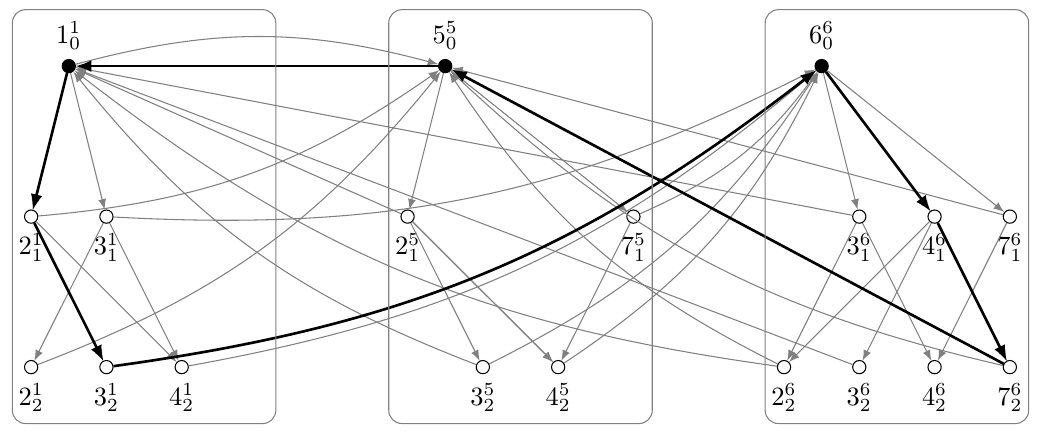
\includegraphics[width=0.8\textwidth]{ejemplo_capas_qb.png}
  \caption{Digrafo en capas $G_{Q B}=\left(V_{Q B}, A_{Q B}\right)$ correspondiente a la instancia dada en la figura \ref{fig:ejemplo_bwtsp}. Las aristas en negrita representan a la solución dada en esa figura. Para ciertos valores de $k$ y $p$ algunos nodos no son alcanzables y no se muestran.}
  \label{fig:ejemplo_capas_qb}
\end{figure}

Al igual que en la formulación dependiente de la posición pura, podemos agregar desigualdades relacionadas a representar el modelo como un digrafo en capas. Estas desigualdades resultan de observar que todos los nodos deben ser alcanzables. En particular, agregamos las ecuaciones \ref{eq:29} determinando que al menos una arista tiene que unir el conjunto de nodos negros con el conjunto que contiene las versiones de un nodo blanco para todos los valores posibles de $k$ y $p$. Llamamos PDPS$^{++}$ al modelo resultante de agregar estas inecuaciones a las de PDPS$^{+}$.

\begin{align}
	& Y\left(\delta^{-}(S)\right) \geq 1 & \forall S \subseteq V_{\mathrm{QB}} \backslash\{j_{0}^{j} : j \in B\},\ \exists i \in W\ |\ \{i_{p}^{k},\ k \in B,\ p \in\{1,2, \ldots, Q\}\} \subseteq S \label{eq:29}
\end{align}

\subsection{Modelo 2-dimensional}

Hasta esta sección solamente analizamos modelos que hablan de una solución dividida en segmentos, con cada segmento encabezado por un nodo negro. Ahora, vamos a ver una formulación que también indica la posición relativa del segmento dentro del camino final. Como antes, necesitamos asumir que un nodo negro arbitrario inicia el ciclo, y por lo tanto su segmento es el primero. El modelo se basa en las variables $Z_{i j}^{m, p} \in\{0,1\},\ \forall m \in\{1,2, \ldots,|B|\},\ \forall p \in\{1,2, \ldots, Q+1\},\ \forall(i, j) \in A$, que indican si el arco $(i,j)$ está en la posición $p$ del segmento número $m$ del ciclo.

\begin{align}
	& Z^{1,1}\left(\delta^{+}(1)\right)=1 \label{eq:30} \\
	& \sum_{j \in B \backslash\{1\}} Z^{m, 1}\left(\delta^{+}(j)\right)=1 & \forall m \in\{2,3, \ldots,|B|\} \label{eq:31} \\
	& \sum_{i \in V \backslash\{1\}} \sum_{p=1}^{Q+1} \sum_{(i, 1) \in A} Z_{i 1}^{|B|, p}=1 & \label{eq:32} \\
	& \sum_{i \in V} \sum_{p=1}^{Q+1} \sum_{(i, k) \in A} Z_{i k}^{m, p}=1 & \forall m \in\{2,3, \ldots,|B|\},\ \forall k \in B \backslash\{1\} \label{eq:33} \\
	& Z^{m, p}\left(\delta^{-}(i)\right)=Z^{m, p+1}\left(\delta^{+}(i)\right) & \forall m \in\{1,2, \ldots,|B|\}, \forall p \in\{1,2, \ldots, Q\},\ \forall i \in W \label{eq:34} \\
	& \sum_{m=1}^{|B|} \sum_{p=1}^{Q+1}\left(Z_{i j}^{m, p}+Z_{j i}^{m, p}\right)=x_{e} & \forall e=\{i, j\} \in E \label{eq:35}
\end{align}

Las restricciones \ref{eq:30} y \ref{eq:31} garantizan que exactamente un segmento se inicia con un nodo negro para cada posición $m \in\{1,2, \ldots,|B|\}$. Por otro lado, las ecuaciones \ref{eq:32} y \ref{eq:33} determinan que la arista que termina el segmento $m-1$ llega al nodo de $B$ que va a empezar el segmento $m$. Las ecuaciones \ref{eq:34} fuerzan el orden de los nodos blancos, y, por último, las ecuaciones de \ref{eq:35} relacionan las variables $Z$ con las del primer modelo.

De forma similar al último modelo discutido, las desigualdades que se usan para modelar el camino implícitamente satisfacen las restricciones de salto, y las restricciones de distancia se pueden expresar así:

\begin{align}
	& \sum_{p=0}^{Q} \sum_{e=\{i, j\} \in E} d_{e}\left(Z_{i j}^{m, p}+Z_{j i}^{m, p}\right) \leq L \quad \forall m \in\{1,2, \ldots,|B|\} \label{eq:36}
\end{align}

Reemplazando las restricciones genéricas \ref{eq:4} y \ref{eq:5} del primer modelo por \ref{eq:30}-\ref{eq:36} e incluyendo las definiciones de $Z$ obtenemos la formulación nueva 2PD, a la que denotaremos 2PD$^{+}$ después de incluir \ref{eq:37}-\ref{eq:39} para eliminar ciclos.

\begin{align}
	& Z_{i j}^{m, p} \leq \sum_{h \neq i} Z_{j h}^{m, p+1} & \forall m \in\{1,2, \ldots,|B|\},\ \forall p \in\{1,2, \ldots, Q\},\ \forall e=\{i, j\} \in E, j \in W \label{eq:37} \\
	& Z_{i j}^{m, p} \leq \sum_{h \neq i} Z_{j h}^{m+1,1} & \forall m \in\{1,2, \ldots,|B|-1\},\ \forall p \in\{1,2, \ldots, Q+1\},\ \forall e=\{i, j\} \in E, j \in B \backslash\{1\} \label{eq:38} \\
	& Z_{i 1}^{|B|, p} \leq \sum_{h \neq i} Z_{1 h}^{1,1} & \forall p \in\{1,2, \ldots, Q+1\},\ \forall e=\{i, 1\} \in E \label{eq:39}
\end{align}

Al igual que en los otros modelos dependientes de la posición, se puede definir un grafo por capas $G_{\mathrm{QI}}=\left(V_{\mathrm{QI}}, A_{\mathrm{QI}}\right)$ que lo representa. Agregar la posición de cada segmento presenta la ventaja de que $G_{QI}$ contiene aristas pertenecientes a un único segmento, y desde este hacia el siguiente. Luego, al introducir una “copia artificial"\ del origen, $G_{QI}$ se convierte en acíclico. Para mantener la consistencia con las secciones previas la definición formal de este grafo no considera las copias del origen, a diferencia de su implementación. Formalmente, el conjunto de vértices de $G_{QI}$ tiene todas las instancias posibles de cada nodo $i$, para poder representar sus ubicaciones posibles dentro de los segmentos con $m$, y cada posición $p$ dentro de él. Cada una de estas instancias se nombra como $i_{p}^{m}$. También se incluyen instancias múltiples de los nodos negros, $i_{0}^{m}$, para comenzar los segmentos. Formalmente, tenemos $V_{\mathrm{QI}}=\bigcup_{m=1}^{|B|} V_{\mathrm{QI}}(m)$ y $A_{\mathrm{QI}}=\bigcup_{m=1}^{|B|} A_{\mathrm{QI}}(m)$, donde $V_{\mathrm{QI}}(m)$ representa el conjunto de nodos que puede encontrarse en el segmento $m$, excepto el nodo negro que lo inicia, mientras que $A_{\mathrm{QI}}(m)$ contiene todas las aristas que podrían pertenecer al segmento $m$. Luego:

$$V_{\mathrm{QI}}(1)=\{1_{0}^{1}\} \cup\{i_{p}^{1}\ |\  i \in W,\ p \in\{1,2, \ldots, Q\} \}$$

$$V_{\mathrm{QI}}(m)=\{i_{0}^{m}\ |\ i \in B \backslash\{1\}\} \cup\{i_{p}^{m}\ |\ i \in W,\ p \in\{1,2, \ldots, Q\}\},\ m \in \{2,3, \ldots,|B|\}$$


\begin{multline*}
	A_{\mathrm{QI}}(m)=\{(i_{p}^{m}, j_{p+1}^{m})\ |\ \{i_{p}^{m},\ j_{p+1}^{m}\} \subseteq V_{\mathrm{QI}}(m),(i, j) \in A\}\ \cup \\ \{(i_{p}^{m},\ j_{0}^{(m+1)})\ |\  i_{p}^{m} \in V_{\mathrm{QI}}(m),\ j_{0}^{(m+1)} \bmod (|B|+1) \in V_{\mathrm{QI}}((m+1) \bmod (|B|+1)),\ (i, j) \in A \}
\end{multline*}

\begin{figure}[H]
  \centering
  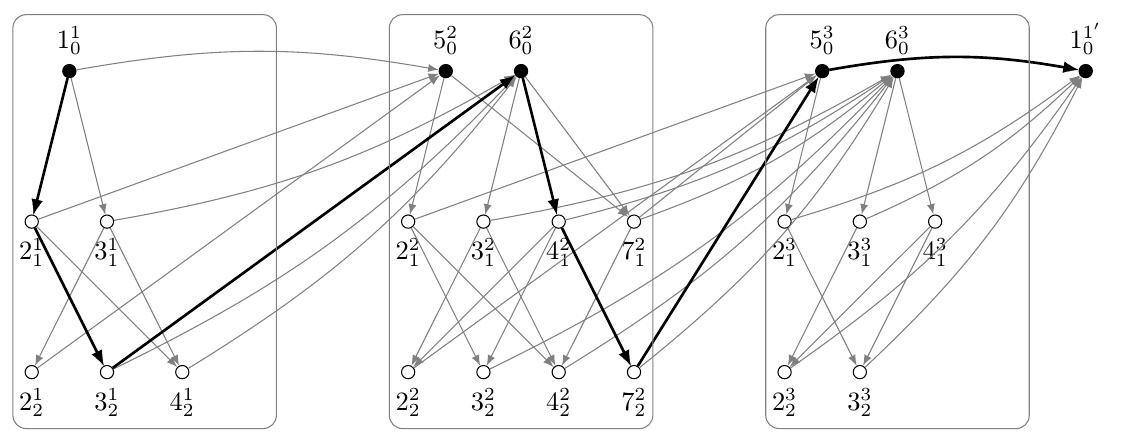
\includegraphics[width=0.8\textwidth]{ejemplo_capas_qi.png}
  \caption{Digrafo en capas $G_{QI}=(V_{QI}, A_{QI})$ correspondiente a la instancia dada en la figura \ref{fig:ejemplo_bwtsp}. Las aristas en negrita representan a la solución dada en esa figura. Para ciertos valores de $m$ y $p$ algunos nodos no son alcanzables y no se muestran. El nodo $1_{0}^{1 \prime}$ es una copia artificial de $1_{0}^{1}$ que se incluye para mejorar la representación visual del grafo.}
  \label{fig:ejemplo_capas_qi}
\end{figure}

El grafo $G_{QI}$ se definió incluyendo todas las instancias posibles de los nodos blancos. Sin embargo, en la implementación hecha por los autores del trabajo original, el grafo se construye incrementalmente, por lo que sólo contiene los vértices y aristas alcanzables desde al menos un nodo negro inicializador de un segmento. Esta estrategia, junto con rutinas de preprocesamiento, genera grafos mucho menores cuando el original es esparzo.

De nuevo, considerando que cada nodo blanco debe poder alcanzarse desde algún nodo negro mediante un camino formado por nodos blancos, se definen las restricciones \ref{eq:40} basadas en la representación del modelo como un grafo de capas. Vamos a llamar 2PD$^{++}$ a la formulación resultante.

\begin{multline}
	 Z(\delta^{-}(S)) \geq 1 \quad \quad \forall S \subseteq V_{\mathrm{QI}} \backslash\{i_{0}^{m}\ |\ i \in B,\ m \in\{1,2, \ldots,|B|\}, \\
	 \exists i \in W : \{i_{p}^{m}\ |\ p \in \{1,2, \ldots, Q\},\ m \in \{1,2, \ldots,|B|\}\} \subseteq S \label{eq:40}
\end{multline}

\section{Modelos alternativos dependientes del tiempo}

Todos los modelos que fueron introducidos en las secciones previas se basan en variables que determinan la posición de las aristas en los distintos segmentos que forman el camino. La definición de estas variables permite cumplir implícitamente las restricciones de salto, mientras que las restricciones de distancia se garantizan con ecuaciones adicionales. Se puede ver que modelos similares pueden ser obtenidos con variables que representan la distancia de las aristas dentro de cada segmento y así aseguran implícitamente que la distancia no se exceda del límite $L$. En este caso, entonces, las restricciones de salto se aseguran agregando restricciones de una manera similar a las restricciones de distancia de los modelos previos.

DD, DDPS y 2DD se pueden obtener modificando los modelos previos dependientes de la posición. DD se basa en las variables $\hat{X}_{ij}^{d} \in \{0,1\},\ d \in \{1,2,\dots,L\},\ \forall(i,j) \in A$ que indican si un camino a $j$ desde el nodo negro previo usando la arista $(i,j)$ tiene una distancia total de $d$. Por otra parte, DDPS usa variables como $\hat{Y}_{ij}^{k,d} \in \{0,1\},\ \forall k \in B,\ \forall d \in \{1,2,\dots,L\},\ \forall (i,j) \in A$, determinando implícitamente la distancia del nodo $j$ en el camino desde el nodo $k$, si la arista $(i,j)$ es parte del camino final. Por último, la representación 2DD hace uso de variables como $\hat{Z}_{ij}^{m,d} \in \{0,1\},\ \forall m \in \{1,2,\dots,|B|\},\ \forall d \in \{1,2,\dots,L\},\ \forall(i,j)\ \in A$, que indican la longitud de los caminos hacia cada vértice después del nodo negro $m$. Las variantes DD$^{+}$, DDPS$^{+}$ y 2DD$^{+}$ se construyen agregando las versiones modificadas apropiadamente de las restricciones para eliminar ciclos definidas previamente. También analizamos DD$^{++}$, DDPS$^{++}$ y 2DD$^{++}$, adaptando las representaciones con grafos de capas a estos casos, e incluyendo los cortes, apropiadamente redefinidos, basados en estas representaciones.

El modelo PDDD se basa en unir, eliminando ecuaciones redundantes, las restricciones de PD y las de DD. Los dos conjuntos de variables, $X$ y $\hat{X}$, se relacionan a través de $x$ del modelo base, y también se extiende para formar PDDD$^{+}$ y PDDD$^{++}$.

Por último, en el trabajo original también se incluye el modelo 3PD que combina información sobre la posición de las aristas y su distancia al principio del segmento. Es decir, usa las variables $X_{ij}^{p,d},\ \forall p \in \{1,2,\dots,Q+1\},\ \forall d \in \{1,2,\dots,L\},\ \forall (i,j) \in A$, que hacen explícitas la posición y la distancia de las aristas dentro de su segmento del camino. De nuevo, 3PD$^{+}$ y 3PD$^{++}$ se construyen como en el caso de los modelos previos.

\section{Comparaciones teóricas}

No se pueden establecer relaciones de dominancia entre muchos de los modelos propuestos porque incorporan conjuntos diferentes y no relacionados de restricciones para modelar los requerimientos del problema. Sin embargo, en algunos casos es posible establecer relaciones basadas en “sentido común"\ acerca de los modelos dependientes de la posición. Antes de comentar estas relaciones vamos a introducir notación necesaria.

Para un modelo $M$, $P(M)$ va a denotar al poliedro inducido por su relajación lineal, y $proj_{x}(P(M))$ a la proyección ortogonal del polinomio $P(M)$ al espacio formado por las variables que representan aristas no dirigidas, que fueron introducidas en el modelo base.

Además, un modelo $M$ se puede considerar como:

\begin{itemize}
	\item \textit{al menos tan fuerte} como el modelo $M'$ si $proj_{x}(P(M)) \subseteq proj_{x}(P(M'))$ vale para todas las instancias;
	\item \textit{más fuerte} que $M'$ si $proj_{x}(P(M)) \subseteq proj_{x}(P(M'))$ vale para todas las instancias y existe al menos una para la que la inclusión es estricta;
	\item \textit{incomparable} a $M'$ si existen instancias para las que $proj_{x}(P(M)) \subseteq proj_{x}(P(M'))$ vale, e instancias para las que $proj_{x}(P(M')) \subseteq proj_{x}(P(M))$ vale.
\end{itemize}

A efectos de poder comparar modelos, vamos a considerar un reformulación de PDPS, PDPS', que se obtiene reemplazando las restricciones de distancia \ref{eq:26} por las restricciones que eliminan caminos de PD reescritas con la variable $Y$ en las ecuaciones \ref{eq:25}. De una manera similar se podría obtener 2PD', a partir de 2PD, reemplazando las restricciones de distancia \ref{eq:36} por lo mismo que en el modelo anterior pero en las ecuaciones \ref{eq:35}. En el trabajo original remarcan que los experimentos computacionales indican que PDPS es significativamente más fuerte en la práctica que PDPS', por lo que no lo consideramos en el resto del texto.

Como comentamos tres párrafos atrás, en algunos casos es posible establecer relaciones, y estas son:

% 1
\begin{theorem}
	PDPS es más fuerte que PS.
\end{theorem}

% 2
\begin{theorem}
	PDPS' es al menos tan fuerte como PD.
\end{theorem}

% 3
\begin{theorem}
	2PD' es al menos tan fuerte como PD.
\end{theorem}

% 4
\begin{theorem}
	PDDD es más fuerte que PD.
\end{theorem}

% 5
\begin{theorem}
	3PD es más fuerte que PDDD.
\end{theorem}

El teorema 1 vale porque PDPS es una reformulación de PS dependiente de la posición.

Resultados análogos a los de los teoremas 4 y 5 se pueden expresar para formulaciones alternativas que implícitamente garantizan las restricciones de distancia, y que usan tipos diferentes de ecuaciones para modelar las restricciones de salto.

\section{Algoritmos}
  
Para implementar los modelos propuestos, los autores del trabajo original desarrollan algoritmos de branch and cut basados en IBM ILOG CPLEX\cite{cplex}.

En las próximas secciones $\overline{x}$, $\overline{X}$ y demás variables de la misma forma, van a denotar a las relajaciones lineales de $x$ y $X$, respectivamente.
  
\subsection{Pre-procesamiento}

Antes de ejecutar el algoritmo se aplica un procesamiento basado en computar el número mínimo de nodos blancos $Q_{min}$ que puede estar contenido en cualquier camino entre dos nodos negro sucesivos. Este mínimo se obtiene para un camino cuando todos los otros contienen $Q$ nodos y si $|W| > Q \times (|B| - 1)$, y es cero en caso contrario:

$$
Q_{min} = max\{0,\ |W|\ -\ Q \times (|B| - 1)\}
$$

Este valor se usa para fijar una cota inferior al lado izquierdo de las restricciones de salto, porque las restricciones de salto modeladas establecen únicamente cotas superiores para su lado izquierdo. También se usa para las variables de PD que indicarían segmentos demasiado cortos: $X_{ij}^{p} = 0$ cuando $j \in B$ para todos los $p \leq Q_{min}$. Es decir, no puede haber una arista que llegue a un nodo negro en una posición del segmento menor a $Q_{min}$ porque esa es la cantidad mínima de nodos blancos entre cada par de nodos negros. Las variables dependientes de la posición de PDPS, 2PD, PDDD y 3PD se limitan de una forma similar.

\subsection{Algoritmo de plano de corte}

Los conjuntos de desigualdades siguientes no se incluyen inicialmente en los modelos, pero se agregan dinámicamente como planos de corte.

Se buscan desigualdades que no valgan en el orden dado a continuación, en caso de que se identifique al menos un corte así en el conjunto se resuelve la relajación lineal, y se continúa con el siguiente conjunto. Podemos decir que una desigualdad “no vale"\ si reduce el tamaño del polítopo actual que representa el problema.

\begin{itemize}
	\item Violaciones a las restricciones de conectividad \ref{eq:3} se encuentran mediante cálculos de flujo máximo en un grafo con sus capacidades basadas en la solución $\overline{x}$ actual.
	\item Las restricciones que eliminan caminos inválidos \ref{eq:18} solamente se agregan para soluciones enteras, porque cuando se aplican a soluciones fraccionarias se agregan demasiadas desigualdades que no valen. A esta altura del procedimiento las soluciones enteras ya son ciclos TSP, por lo que encontrar caminos inviables se puede hacer en tiempo lineal.
	\item Las desigualdades de balanceo de flujo \ref{eq:9}, \ref{eq:16}, \ref{eq:24} y \ref{eq:34} se separan por enumeración.
	\item De la misma forma que en el punto anterior se separan las restricciones que eliminan ciclos \ref{eq:19}, \ref{eq:20}, \ref{eq:27}, \ref{eq:28}, \ref{eq:37}, \ref{eq:38} y \ref{eq:39}.
	\item Los cortes basadas en las representaciones como grafos de capas de los modelos \ref{eq:21}, \ref{eq:29} y \ref{eq:40}, se separan como los de conectividad \ref{eq:3}. La diferencia principal es que hay que garantizar que todas las copias de al menos nodo blanco estén en el conjunto de soluciones posibles, lo que se garantiza asignando capacidades altas a las aristas desde todas las copias de un nodo blanco en particular a un sumidero artificial. Se quiere garantizar esta condición para contar con al menos una solución candidata para cada ubicación posible de un nodo blanco. % NO ESTOY SEGURA DE QUE ESA EXPLICACIÓN ESTÉ BIEN
\end{itemize}

Para manejar el gran número de desigualdades y la convergencia lenta de los planos de corte, se aplican las siguientes reglas:

\begin{itemize}
	\item Supongamos que una desigualdad válida en un grafo de capas $G_{Q}$ tiene la forma $\overline{X}(A) \geq b$. Solamente agregamos el corte si $\overline{X}(A) < \Delta \times b$ con $\Delta \in (0,1]$.
	\item Si el valor de la relajación lineal no aumenta en las últimas cinco iteraciones de los planos de corte en un nodo de branch and bound se continúa con la ramificación.
	\item Después de resolver un problema de flujo máximo para buscar conjuntos de cortes violados podríamos obtener soluciones múltiples. En ese caso, consideramos las soluciones que generan el conjunto menor y el mayor, y agregamos también la que tiene el número mínimo de cortes.
\end{itemize}

\subsection{Heurísticas}

Las cotas son esenciales para podar el árbol de branch and bound, y en este trabajo también decidieron usar heurísticas en cada nodo del árbol. Estas heurísticas se llaman después de cada iteración de corte en la raíz, en uno de cada cinco nodos dentro de los primeros 100, en uno de cada 25 en los primeros 1000, en uno de cada 100 en los primeros 5000, y en uno de cada 500 en el resto.

Para construir soluciones factibles aplican una heurística de vecinos más cercanos guiada por la solución lineal del nodo actual. El camino se extiende paso por paso eligiendo el sucesor no visitado más “barato"\ que cumple las condiciones de salto pero no necesariamente las de distancia. Para esto también se considera el número mínimo de nodos blancos después de cada nodo negro $Q_{min}$.

Para arreglar y mejorar una solución, corren una variante de GVNS \cite{gvns}. VNS es una metaheurística para resolver problemas de optimización. Explora vecindarios distantes de la solución actual y se mueve a uno nuevo solamente si se obtiene una mejora. Mientras que GVNS es una variante de VNS que usa VND para las búsquedas locales. VND es una variante de VNS que cambia de vecindario de forma determinística. Con una probabilidad de 0.5 se elije la mejor solución global como inicio en una iteración de GVNS, en caso contrario se usa la mejor solución encontrada en la ejecución actual de la heurística. Para mejorar localmente la solución, VND hace dos tipos de cambios:

\begin{itemize}
	\item Mueve un nodo a otra posición del ciclo.
	\item Intercambia la posición de dos vértices.
\end{itemize}

En cada iteración de VND se buscan movimientos en ambos vecindarios, para reducir las distancias si esa restricción todavía no se cumple, o para mejorar la calidad de la solución. Se elije aleatoriamente entre los cinco mejores movimientos, valorando más acercarse a cumplir las restricciones de distancia que mejorar el costo. Para diversificar la solución en GVNS se aplican $\lceil 0.05 \times |V| \rceil$ intercambios aleatorios, manteniendo la viabilidad de los saltos y sin aumentar las distancias inválidas. Si después de dos iteraciones de GVNS no se mejora la solución global entonces se aumenta en uno la cantidad de nodos que se intercambian, hasta  $\lceil 0.3 \times |V| \rceil$ como máximo. La heurística termina si después de 20 iteraciones de GVNS no se encuentra una solución mejor. Las soluciones finales que no cumplen con las ecuaciones de distancia se abandonan, pero es algo que casi no se vio en las experimentaciones.

\section{Resultados empíricos}

(Por ahí habría que mejorar este título)

\subsection{Instancias}

\subsection{Relajaciones}

\subsection{Análisis de los resultados}

\pagebreak

\begin{thebibliography}{9}

\bibitem{main}
L. Gouveia, M. Leitner y M. Ruthmair, “Extended formulations and branch-and-cut algorithms for the Black-and-White Traveling Salesman Problem". European Journal of Operational Research, 262-3, 908-928. 2017.

\bibitem{ip_tutorial}
G. Cornuéjols, M. Trick y M. Saltzman, “A tutorial on integer programming". CMU Technical Report. 1995.

\bibitem{teaching_ip_tsp}
G. Pataki, “Teaching integer programming formulations using the traveling salesman problem". SIAM Review 45-1, 116-123. 2003.

\bibitem{branch_and_cut}
J. E. Mitchell, “Branch-and-Cut Algorithms for Combinatorial Optimization Problems". 2002.

\bibitem{branc_and_bound}
J. Clausen, “Branch and Bound Algorithms—Principles and Examples". 1999.

\bibitem{cplex}
IBM ILOG CPLEX Optimization Studio. URL: \url{https://www.ibm.com/es-es/products/ilog-cplex-optimization-studio}. [En línea, accedido el 23 de abril de 2019.]

\bibitem{gvns}
P. Venkatesh, G. Srivastava y A. Singh, “A general variable neighborhood search algorithm for the k-traveling salesman problem". 2018.

\end{thebibliography}

\end{document}